\documentclass[twocolumn,11pt]{abst}
\usepackage{url}
\usepackage{listings}
\usepackage{float}
\setlength\intextsep{5pt}
\setlength\textfloatsep{5pt}

\lstset{%
  language={C},
  basicstyle={\small},%
  identifierstyle={\small},%
  commentstyle={\small\itshape},%
  keywordstyle={\small\bfseries},%
  ndkeywordstyle={\small},%
  stringstyle={\small\ttfamily},
  frame={tb},
  breaklines=true,
  columns=[l]{fullflexible},%
  numbers=left,%
  xrightmargin=0zw,%
  xleftmargin=3zw,%
  numberstyle={\scriptsize},%
  stepnumber=1,
  numbersep=1zw,%
  lineskip=-0.5ex%
}

% タイトル
\title{データロギングシステムの研究}

\author{藤井岳寛(指導教員 伊藤恒平,林道大)}

%\urlstyle{rm}

\setcounter{page}{33}
\lhead{}
\chead{}
\rhead{{\sf 17・217}\\{\bf 機械工学科}}
\lfoot{}
\cfoot{{\sf-\ M-\thepage \ -}}
%\rfoot{}
\renewcommand{\headrulewidth}{3pt}
%\renewcommand{\footrulewidth}{1pt}



\begin{document}
%\layout
\maketitle
\thispagestyle{fancy}
\pagestyle{fancy}

\setlength{\baselineskip}{5.6truemm}
\kanjiskip=.07zw plus 3pt minus 3pt
\xkanjiskip=.07zw plus 3pt minus 3pt


% 本文

\section{緒言}
\subsection{研究の背景}
本研究室では毎年高専ロボコンに参加し,昨年まで3年連続で全国大会に出場している.
今年は地区大会を優勝し,全国大会に出場することを目標とした.
試合に勝つための作戦を考え,その作戦を実行できるロボットを設計・製作した.
しかし,地区大会初戦で原因不明のマシントラブルに見舞われ敗退した.
原因不明というのは,1)試合後は正常に動作し現象が再現されないこと.
2)ロボットのデータログを記録していなかったため,状況を再現して検証が行えないこと.
学校での動作試験でも原因不明の不具合に幾度が見舞われたが,
現象を再現できず,対応に遅れ結果的にロボット完成が遅れた.
これらのことから,ロボットのデータログを記録していれば多くの不具合を修正でき,
上位入賞できたのではないかと考える.


\subsection{研究の目的}
今まではロボットの制御システムから設計を始め,マイコンの選定などを行ってきた.
しかし,毎回そこから始めるのは大変で,時間がかかるため効率的ではない.
今回ロボットの制御に使用した,Arduinoはユーザーの作ったライブラリがたくさんあるため
プログラムの開発には便利である.しかし,機能を追加するにはShieldと呼ばれる基盤を重ねなければならないのは不便である.
そのため,USBhostやSDカードソケットなどを備えていてArduinoに似た開発環境を使える
GR-SAKURAをメインとしたロボットのデータログを記録する機能を備えたロボット制御システムと
仕様や導入方法をまとめたマニュアルを作成し,来年度以降の活動を支援する.


\section{メインマイコンの選定}
今回はArduinoMegaをメインとして使用した制御システムを構成したが,
本当にロボコンにふさわしいマイコンは何なのかを再検討する.
今年度のロボットをもとにマイコンに要求される項目を表\ref{spec}にまとめる.
\begin{table}[htb]
 \begin{center}
  \caption{要求スペック}
  \scalebox{0.6}{
  \begin{tabular}[htbp]{|c|c|p{9cm}|}
  \hline
  項目 & 数 & 理由 \\
  \hline
  デジタルIO & 16 & ソレノイドやLEDを使うのに多く必要 \\
  \hline
  アナログIO & 4 & アナログデータが必要なアクチュエータやセンサをする場合に必要 \\
  \hline
  PWMピン & 16 & サーボモータの制御に使うため \\
  \hline
  シリアルポート & 4 & 今年度は3輪オムニの制御に3つ使用したが,4輪メカナムや4輪オムニなどを使用するには4つ必要である \\
  \hline
  SDカードソケット & 1 & データログを記録するためにSDカード使う \\
  \hline
  USBホスト & 1 & Bluetoothドングルを使いBluetooth通信するため \\
  \hline
  \end{tabular}
  }
    \label{spec}
 \end{center}
\end{table}

\subsection{Arduinoの性能比較}
今回の高専ロボコンではライブラリが豊富であり比較的開発が簡単であるArduinoシリーズの中で
Serialポートが3つあるArdinoMegaを使用したが,Arduinoの性能を調べ比較してみる.
各Arduinoの性能をまとめた表\ref{arduino}を下に示す.



\begin{table}[htb]
 \begin{center}
  \caption{Arduinoスペック一覧}
  \scalebox{0.45}{
  \begin{tabular}[htbp]{|c|c|c|c|c|c|}
  \hline
  名前 & ArduinoUNO & Arduino101 & ArduinoPRO & ArduinoProMini & ArduinoMega2560  \\
  \hline
  大きさ & 68.6$\times$53.4mm & 68.6$\times$53.4mm & 43$\times$18mm & 101.52$\times$53.3mm & 56$\times$25mm  \\
  \hline
  重さ & 25g & & 9g & & 37g  \\
  \hline
  価格 & 3200 & 4980 & 1868 & 1243 & 5830 \\ 
  \hline
  マイコン & ATmega328P & InrelCurie & ATmega328 & ATmega328 & ATmega2560   \\
  \hline
  動作電圧 & 5V & 3.3V & 3.3or5V & 5V & 3.3or5V  \\
  \hline
  電源電圧 & 7-20V & 7-20V & 3.35-12V & 3.35-12V & 6-20V \\ 
  \hline
  デジタルIO & 14 & 14 & 14  & 14 & 54  \\
  \hline
  アナログIO & 6 & 6 & 6 & 8 & 16  \\
  \hline
  pwmピン & 6 & 4 & 6 & 6 & 15  \\
  \hline
  シリアルポート & 1 & 1 & 1 & 1 & 4  \\
  \hline
  フラッシュメモリ & 32kB & 196kB & 32kB & 32kB & 256kB  \\
  \hline
  SRAM & 2kB & 24kB & 2kB & 2kB & 8kB  \\
  \hline
  EEPROM & 1kB & & 1kB & 1kB & 4kB  \\
  \hline
  クロック & 16MHz & 32MHz & 8or16MHz & 8or16MHz & 16MHz  \\
  \hline
  \hline
  名前 & ArduinoYUN & ArduinoDUE & ArduinoMegaADK & ArduinoEthrnet & ArduinoLeonardo  \\
  \hline
  大きさ & 101.52$\times$53.3mm & 101.52$\times$53.3mm & 68.6$\times$53.3mm & 68.6$\times$53.4mm & 28$\times$65mm \\
  \hline
  重さ & 36g & 36g & 28g & 20g & 9g \\
  \hline
  価格 & 9990 & 6264 & 8208 & 7676 & 3132  \\
  \hline
  マイコン & ATmega32U4 & AT91SAM3X8E & ATmega2560 & ATmega328 & ATmega32U4 \\
  \hline
  動作電圧 & 5V & 3.3V & 5V & 5V & 5V \\
  \hline
  電源電圧 & 5V & 6-16V & 6-20V & 6-20V & 7-12V \\
  \hline 
  デジタルIO & 20 & 54 & 54 & 14 & 20 \\
  \hline 
  アナログIO & 12 & 12 & 16 & 6 & 12 \\
  \hline
  pwmピン & 7 & 12 & 15 & 5 & 7  \\
  \hline
  シリアルポート & 1 & 4 & 4 & 1 & 1  \\
  \hline 
  フラッシュメモリ & 32kB & 256kB & 256kB & 32kB & 32kB  \\
  \hline
  SRAM & 2.5kB & 96kB & 8kB & 2kB & 2.5kB  \\
  \hline
  EEPROM 1kB & & 4kB & 1kB & 1kB & 1kB \\
  \hline
  16MHz & 84MHz & 16MHz & 16MHz & 16MHz & 16MHz \\
  \hline
  \end{tabular}
  }
    \label{arduino}
 \end{center}
\end{table}


\subsection{GRシリーズ}
より汎用性の高いGRシリーズのスペックをまとめ検討する.
GRシリーズの性能をまとめた表\ref{GR}を下に示す.
\begin{table}[htb]
 \begin{center}
  \caption{GRスペック一覧}
  \scalebox{0.65}{
  \begin{tabular}[htbp]{|c|c|c|c|}
  \hline
  名前 & GR-SAKURA & GR-KAEDE & GR-PEACH \\
  \hline
  大きさ & 53.34$\times$65.58mm & 53.84$\times$91.83mm & 53.84$\times$67.58mm \\
  \hline
  価格 & 4640 & 7500 & 9690 \\
  \hline
  マイコン & RX63N & RX64N & RZ/A1H \\
  \hline
  動作電圧 & 3.3V & 3.3V & 3.3V \\
  \hline
  電源電圧 & 5V & 5V & 5V \\
  \hline
  デジタルIO & 55 & 29 & 52 \\
  \hline
  アナログIO & 16 & 12 & 6 \\
  \hline
  pwmピン & 9 & 9 & 6 \\
  \hline
  シリアルポート & 4 & 4 & 7 \\
  \hline
  フラッシュメモリ & 32kB & 64kB & 8MB \\
  \hline
  SRAM & 128kB & 552kB & 10MB \\
  \hline
  EEPROM & 1MB & 4MB & 8MB \\
  \hline
  クロック & 96MHz & 96MHz & 400MHz \\
  \hline
  \end{tabular}
  }
    \label{GR}
 \end{center}
\end{table}

\subsection{GR-SAKURA}
GR-SAKURA FULLをメインマイコンに選定した.
GR-SAKURAは豊富なIOに加えてLANコネクタ,USBホストコネクタ,SDカードソケットを備えている.
GR-SAKURAを図\ref{fig:sakura}に示す.\\

\begin{figure}[h]
 \begin{center}
  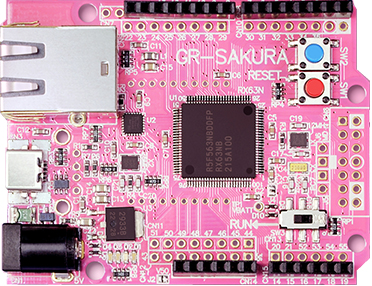
\includegraphics[width=50mm]{sakurafull.jpg}
 \end{center}
 \caption{GR-SAKURA}
 \label{fig:sakura}
\end{figure}

\section{自作Shieldについて}
\subsection{今年度の構成}
今年度はArduinoMegaにコントローラーと通信するためのUSBhostShieldと
サーボモータを制御するためのServoShieldを載せ,
さらに各種IOを使いやすくするための自作Shieldも搭載した.

\subsection{ロボコンShield}
GR-SAKURAはUSBhostやSDカードソケットが搭載されているため,
シリアル通信の規格をRS485に変換するトランシーバと各種IOを外側に出し,接続しやすくするものを作成する.
ロボコンシールドのブロック図を図\ref{fig:block}に示す.\\

\begin{figure}[H]
 \begin{center}
  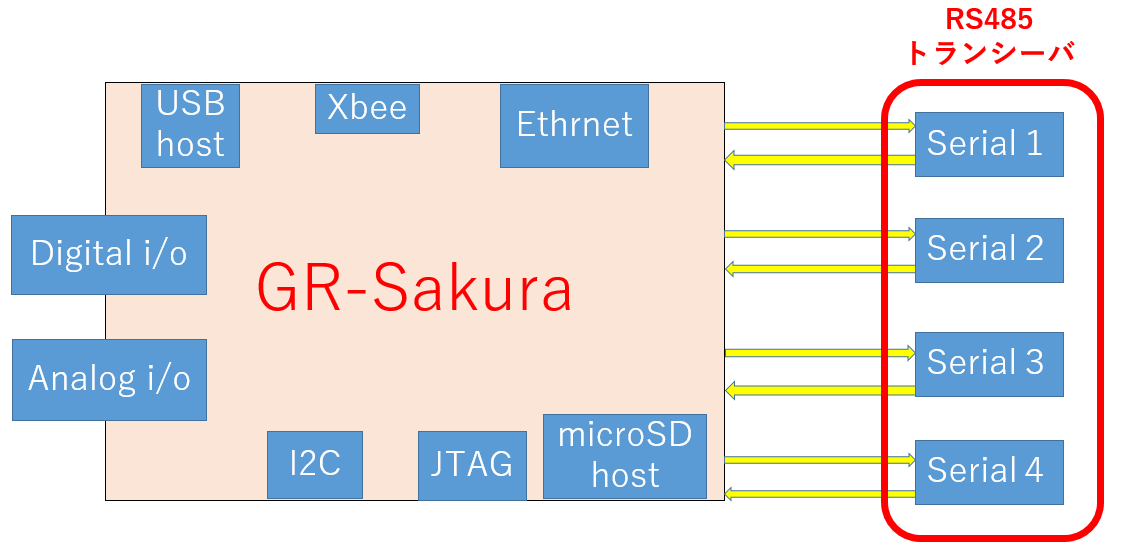
\includegraphics[width=80mm]{block.png}
 \end{center}
 \caption{Shieldブロック図}
 \label{fig:block}
\end{figure}

\section{データログシステム開発}
\subsection{プログラム}

データを記録するメインプログラムと,記録するデータを取得するためのファイルを作成した.
プログラムの機能を以下に示す.
\begin{itemize}
 \item 記録するデータログリストファイルの読み取り
 \item リストにもとづいて必要なデータをログデータとしてまとめる
 \item 必要データを1レコードとして記録する
 \item 1レコードごとにタイムスタンプをつける
 \item レコードごとにテキストファイルとして書き出す
\end{itemize}


\section{結言}

ロボコン標準制御システムの考案にあたり,メインマイコンに豊富なI/OやUSBhost,SDカードソケットが既存で備えられているGR-SAKURAを選定した.
しかし,開発環境はArduinoIDEに似ているIDEforGRを使う予定だったが,現状はオンライン環境のRenesasWebコンパイラを使うしかない.
ログシステムはGR-SAKURAでSDカードにテキストファイルを生成し,データログが書き込まれているのを確認をした.
標準制御システムを考案したことにより開発にかかる時間の短縮,
ログシステムの開発によりデバッグにかかる時間が短縮されロボットの完成度の向上が見込める.

% 参考文献
\begin{thebibliography}{8}


\bibitem{sakura} \url{http://gadget.renesas.com/ja/product/sakura.html}

\end{thebibliography}


\end{document}

○○○○○○○○○○○○○○○○○○○○○○○○○○○○○○○○○○○○○○○○○○○○○○○○
○○○○○○○○○○○○○○○○○○○○○○○○○○○○○○○○○○○○○○○○○○○○○○○○
○○○○○○○○○○○○○○○○○○○○○○○○○○○○○○○○○○○○○○○○○○○○○○○○
○○○○○○○○○○○○○○○○○○○○○○○○○○○○○○○○○○○○○○○○○○○○○○○○
○○○○○○○○○○○○○○○○○○○○○○○○○○○○○○○○○○○○○○○○○○○○○○○○
○○○○○○○○○○○○○○○○○○○○○○○○○○○○○○○○○○○○○○○○○○○○○○○○
○○○○○○○○○○○○○○○○○○○○○○○○○○○○○○○○○○○○○○○○○○○○○○○○
○○○○○○○○○○○○○○○○○○○○○○○○○○○○○○○○○○○○○○○○○○○○○○○○
○○○○○○○○○○○○○○○○○○○○○○○○○○○○○○○○○○○○○○○○○○○○○○○○
○○○○○○○○○○○○○○○○○○○○○○○○○○○○○○○○○○○○○○○○○○○○○○○○
○○○○○○○○○○○○○○○○○○○○○○○○○○○○○○○○○○○○○○○○○○○○○○○○
○○○○○○○○○○○○○○○○○○○○○○○○○○○○○○○○○○○○○○○○○○○○○○○○
○○○○○○○○○○○○○○○○○○○○○○○○○○○○○○○○○○○○○○○○○○○○○○○○
○○○○○○○○○○○○○○○○○○○○○○○○○○○○○○○○○○○○○○○○○○○○○○○○
○○○○○○○○○○○○○○○○○○○○○○○○○○○○○○○○○○○○○○○○○○○○○○○○
○○○○○○○○○○○○○○○○○○○○○○○○○○○○○○○○○○○○○○○○○○○○○○○○
○○○○○○○○○○○○○○○○○○○○○○○○○○○○○○○○○○○○○○○○○○○○○○○○
○○○○○○○○○○○○○○○○○○○○○○○○○○○○○○○○○○○○○○○○○○○○○○○○
○○○○○○○○○○○○○○○○○○○○○○○○○○○○○○○○○○○○○○○○○○○○○○○○
○○○○○○○○○○○○○○○○○○○○○○○○○○○○○○○○○○○○○○○○○○○○○○○○
○○○○○○○○○○○○○○○○○○○○○○○○○○○○○○○○○○○○○○○○○○○○○○○○
○○○○○○○○○○○○○○○○○○○○○○○○○○○○○○○○○○○○○○○○○○○○○○○○
○○○○○○○○○○○○○○○○○○○○○○○○○○○○○○○○○○○○○○○○○○○○○○○○
○○○○○○○○○○○○○○○○○○○○○○○○○○○○○○○○○○○○○○○○○○○○○○○○
○○○○○○○○○○○○○○○○○○○○○○○○○○○○○○○○○○○○○○○○○○○○○○○○
○○○○○○○○○○○○○○○○○○○○○○○○○○○○○○○○○○○○○○○○○○○○○○○○
○○○○○○○○○○○○○○○○○○○○○○○○○○○○○○○○○○○○○○○○○○○○○○○○
○○○○○○○○○○○○○○○○○○○○○○○○○○○○○○○○○○○○○○○○○○○○○○○○
○○○○○○○○○○○○○○○○○○○○○○○○○○○○○○○○○○○○○○○○○○○○○○○○
○○○○○○○○○○○○○○○○○○○○○○○○○○○○○○○○○○○○○○○○○○○○○○○○
○○○○○○○○○○○○○○○○○○○○○○○○○○○○○○○○○○○○○○○○○○○○○○○○
○○○○○○○○○○○○○○○○○○○○○○○○○○○○○○○○○○○○○○○○○○○○○○○○
○○○○○○○○○○○○○○○○○○○○○○○○○○○○○○○○○○○○○○○○○○○○○○○○
○○○○○○○○○○○○○○○○○○○○○○○○○○○○○○○○○○○○○○○○○○○○○○○○
○○○○○○○○○○○○○○○○○○○○○○○○○○○○○○○○○○○○○○○○○○○○○○○○
○○○○○○○○○○○○○○○○○○○○○○○○○○○○○○○○○○○○○○○○○○○○○○○○
○○○○○○○○○○○○○○○○○○○○○○○○○○○○○○○○○○○○○○○○○○○○○○○○
○○○○○○○○○○○○○○○○○○○○○○○○○○○○○○○○○○○○○○○○○○○○○○○○
○○○○○○○○○○○○○○○○○○○○○○○○○○○○○○○○○○○○○○○○○○○○○○○○
○○○○○○○○○○○○○○○○○○○○○○○○○○○○○○○○○○○○○○○○○○○○○○○○
○○○○○○○○○○○○○○○○○○○○○○○○○○○○○○○○○○○○○○○○○○○○○○○○
○○○○○○○○○○○○○○○○○○○○○○○○○○○○○○○○○○○○○○○○○○○○○○○○
○○○○○○○○○○○○○○○○○○○○○○○○○○○○○○○○○○○○○○○○○○○○○○○○
○○○○○○○○○○○○○○○○○○○○○○○○○○○○○○○○○○○○○○○○○○○○○○○○
○○○○○○○○○○○○○○○○○○○○○○○○○○○○○○○○○○○○○○○○○○○○○○○○
○○○○○○○○○○○○○○○○○○○○○○○○○○○○○○○○○○○○○○○○○○○○○○○○
○○○○○○○○○○○○○○○○○○○○○○○○○○○○○○○○○○○○○○○○○○○○○○○○
○○○○○○○○○○○○○○○○○○○○○○○○○○○○○○○○○○○○○○○○○○○○○○○○
○○○○○○○○○○○○○○○○○○○○○○○○○○○○○○○○○○○○○○○○○○○○○○○○
○○○○○○○○○○○○○○○○○○○○○○○○○○○○○○○○○○○○○○○○○○○○○○○○
○○○○○○○○○○○○○○○○○○○○○○○○○○○○○○○○○○○○○○○○○○○○○○○○
○○○○○○○○○○○○○○○○○○○○○○○○○○○○○○○○○○○○○○○○○○○○○○○○
○○○○○○○○○○○○○○○○○○○○○○○○○○○○○○○○○○○○○○○○○○○○○○○○
○○○○○○○○○○○○○○○○○○○○○○○○○○○○○○○○○○○○○○○○○○○○○○○○
○○○○○○○○○○○○○○○○○○○○○○○○○○○○○○○○○○○○○○○○○○○○○○○○
○○○○○○○○○○○○○○○○○○○○○○○○○○○○○○○○○○○○○○○○○○○○○○○○
○○○○○○○○○○○○○○○○○○○○○○○○○○○○○○○○○○○○○○○○○○○○○○○○
○○○○○○○○○○○○○○○○○○○○○○○○○○○○○○○○○○○○○○○○○○○○○○○○
○○○○○○○○○○○○○○○○○○○○○○○○○○○○○○○○○○○○○○○○○○○○○○○○
○○○○○○○○○○○○○○○○○○○○○○○○○○○○○○○○○○○○○○○○○○○○○○○○
○○○○○○○○○○○○○○○○○○○○○○○○○○○○○○○○○○○○○○○○○○○○○○○○
○○○○○○○○○○○○○○○○○○○○○○○○○○○○○○○○○○○○○○○○○○○○○○○○
○○○○○○○○○○○○○○○○○○○○○○○○○○○○○○○○○○○○○○○○○○○○○○○○
○○○○○○○○○○○○○○○○○○○○○○○○○○○○○○○○○○○○○○○○○○○○○○○○
○○○○○○○○○○○○○○○○○○○○○○○○○○○○○○○○○○○○○○○○○○○○○○○○
○○○○○○○○○○○○○○○○○○○○○○○○○○○○○○○○○○○○○○○○○○○○○○○○
○○○○○○○○○○○○○○○○○○○○○○○○○○○○○○○○○○○○○○○○○○○○○○○○
○○○○○○○○○○○○○○○○○○○○○○○○○○○○○○○○○○○○○○○○○○○○○○○○
○○○○○○○○○○○○○○○○○○○○○○○○○○○○○○○○○○○○○○○○○○○○○○○○
○○○○○○○○○○○○○○○○○○○○○○○○○○○○○○○○○○○○○○○○○○○○○○○○
○○○○○○○○○○○○○○○○○○○○○○○○○○○○○○○○○○○○○○○○○○○○○○○○
○○○○○○○○○○○○○○○○○○○○○○○○○○○○○○○○○○○○○○○○○○○○○○○○
○○○○○○○○○○○○○○○○○○○○○○○○○○○○○○○○○○○○○○○○○○○○○○○○
○○○○○○○○○○○○○○○○○○○○○○○○○○○○○○○○○○○○○○○○○○○○○○○○
○○○○○○○○○○○○○○○○○○○○○○○○○○○○○○○○○○○○○○○○○○○○○○○○
○○○○○○○○○○○○○○○○○○○○○○○○○○○○○○○○○○○○○○○○○○○○○○○○
○○○○○○○○○○○○○○○○○○○○○○○○○○○○○○○○○○○○○○○○○○○○○○○○
○○○○○○○○○○○○○○○○○○○○○○○○○○○○○○○○○○○○○○○○○○○○○○○○
○○○○○○○○○○○○○○○○○○○○○○○○○○○○○○○○○○○○○○○○○○○○○○○○
○○○○○○○○○○○○○○○○○○○○○○○○○○○○○○○○○○○○○○○○○○○○○○○○
○○○○○○○○○○○○○○○○○○○○○○○○○○○○○○○○○○○○○○○○○○○○○○○○
○○○○○○○○○○○○○○○○○○○○○○○○○○○○○○○○○○○○○○○○○○○○○○○○
○○○○○○○○○○○○○○○○○○○○○○○○○○○○○○○○○○○○○○○○○○○○○○○○
○○○○○○○○○○○○○○○○○○○○○○○○○○○○○○○○○○○○○○○○○○○○○○○○
○○○○○○○○○○○○○○○○○○○○○○○○○○○○○○○○○○○○○○○○○○○○○○○○
○○○○○○○○○○○○○○○○○○○○○○○○○○○○○○○○○○○○○○○○○○○○○○○○
○○○○○○○○○○○○○○○○○○○○○○○○○○○○○○○○○○○○○○○○○○○○○○○○
○○○○○○○○○○○○○○○○○○○○○○○○○○○○○○○○○○○○○○○○○○○○○○○○
○○○○○○○○○○○○○○○○○○○○○○○○○○○○○○○○○○○○○○○○○○○○○○○○
○○○○○○○○○○○○○○○○○○○○○○○○○○○○○○○○○○○○○○○○○○○○○○○○
○○○○○○○○○○○○○○○○○○○○○○○○○○○○○○○○○○○○○○○○○○○○○○○○
○○○○○○○○○○○○○○○○○○○○○○○○○○○○○○○○○○○○○○○○○○○○○○○○
○○○○○○○○○○○○○○○○○○○○○○○○○○○○○○○○○○○○○○○○○○○○○○○○
○○○○○○○○○○○○○○○○○○○○○○○○○○○○○○○○○○○○○○○○○○○○○○○○
○○○○○○○○○○○○○○○○○○○○○○○○○○○○○○○○○○○○○○○○○○○○○○○○
○○○○○○○○○○○○○○○○○○○○○○○○○○○○○○○○○○○○○○○○○○○○○○○○
○○○○○○○○○○○○○○○○○○○○○○○○○○○○○○○○○○○○○○○○○○○○○○○○
○○○○○○○○○○○○○○○○○○○○○○○○○○○○○○○○○○○○○○○○○○○○○○○○
○○○○○○○○○○○○○○○○○○○○○○○○○○○○○○○○○○○○○○○○○○○○○○○○
○○○○○○○○○○○○○○○○○○○○○○○○○○○○○○○○○○○○○○○○○○○○○○○○
○○○○○○○○○○○○○○○○○○○○○○○○○○○○○○○○○○○○○○○○○○○○○○○○
○○○○○○○○○○○○○○○○○○○○○○○○○○○○○○○○○○○○○○○○○○○○○○○○
○○○○○○○○○○○○○○○○○○○○○○○○○○○○○○○○○○○○○○○○○○○○○○○○
○○○○○○○○○○○○○○○○○○○○○○○○○○○○○○○○○○○○○○○○○○○○○○○○


